\section{AlphaFold2 Characteristics and Bottleneck Analysis}
\label{sec:analysis}

To identify the optimization opportunities and design constraints relevant to OPA-equipped CPUs, we first review the structure of AlphaFold2 and then quantify three system-level bottlenecks: dense GEMM computation, activation-dominated memory pressure, and frequent tensor-layout transformations. %The analysis proceeds top-down---from the overall model, to the workload breakdown across modules, to a detailed characterization of the dominant kernels.

\subsection{AlphaFold2 Model Overview}
\label{sec:analysis:model}

\begin{figure*}[t]
    \centering
    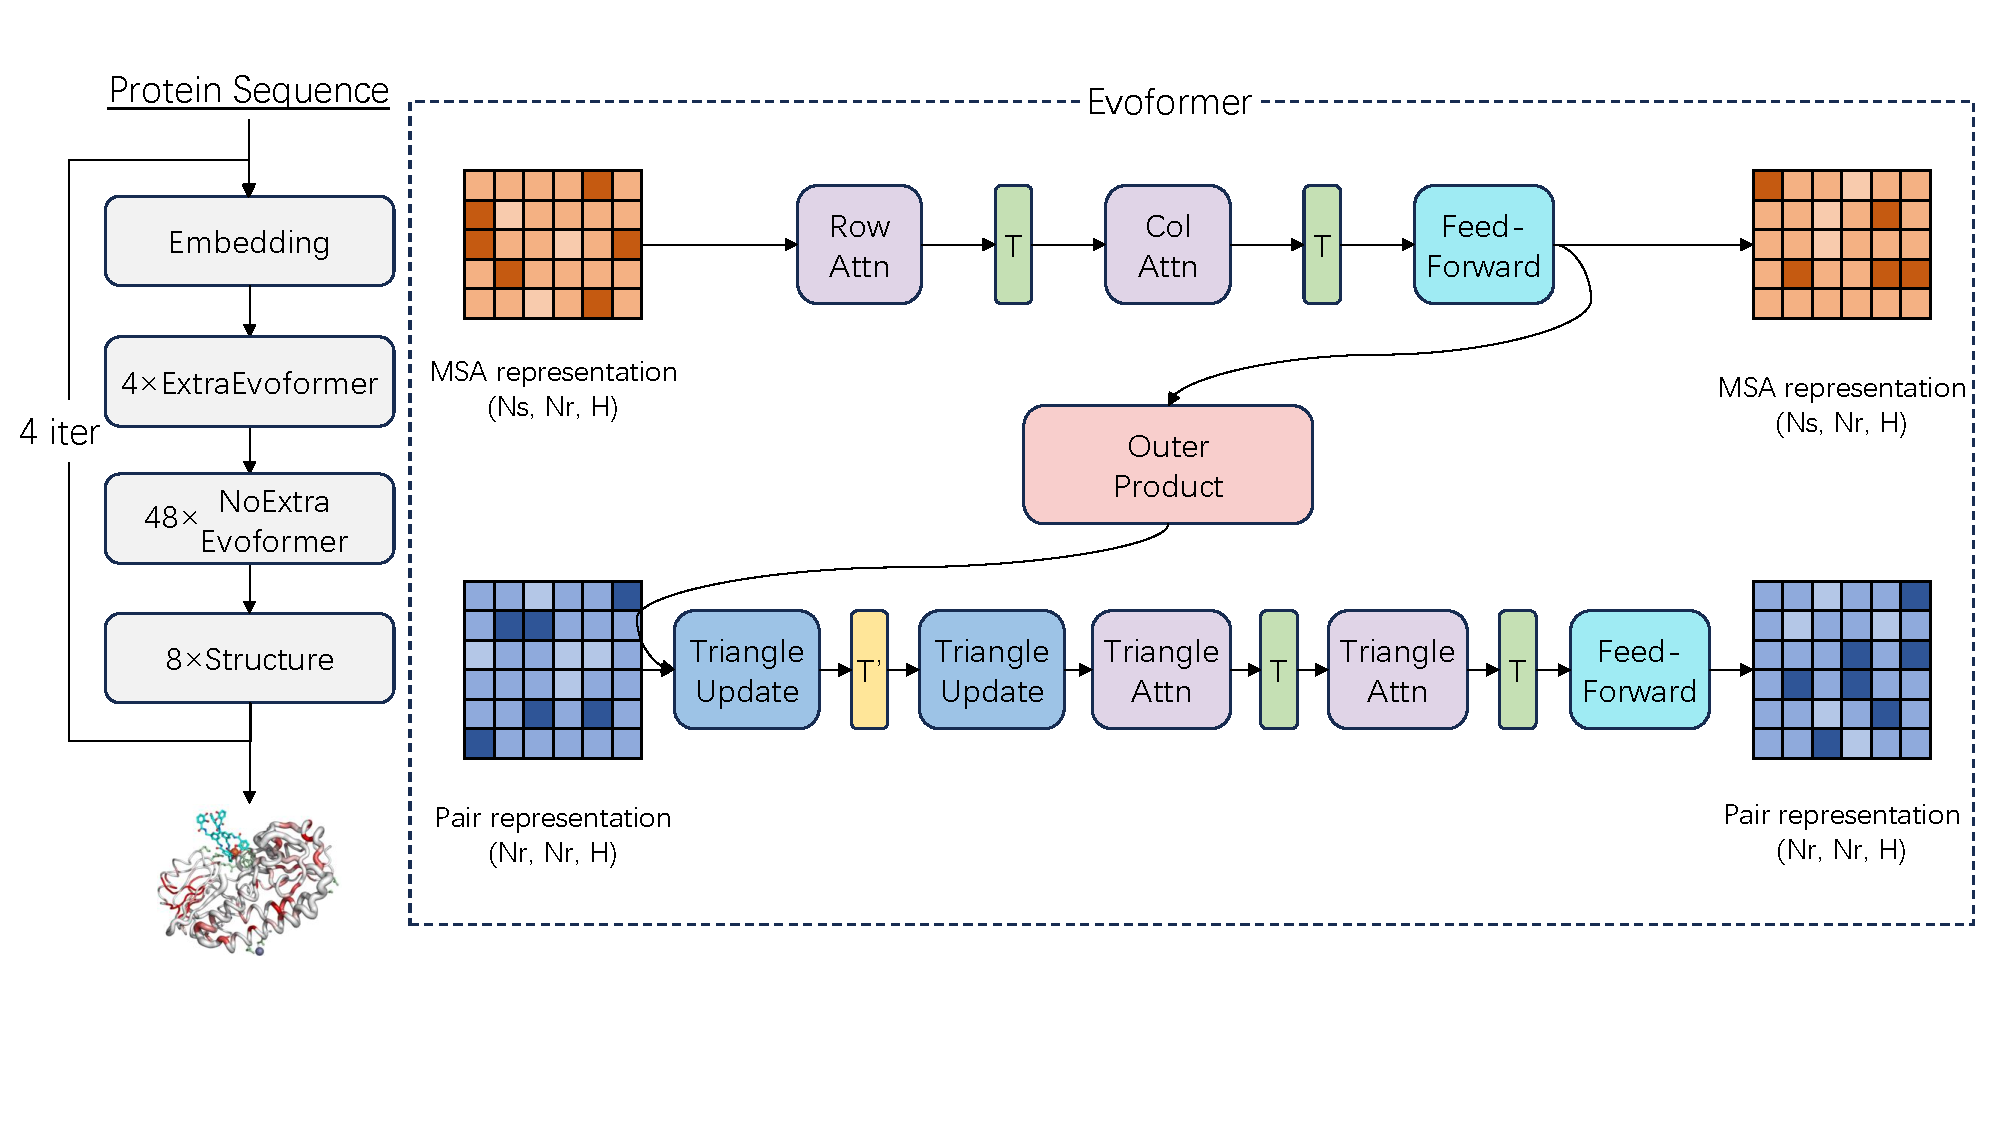
\includegraphics[width=0.95\textwidth]{figures/AlphaFold.pdf}
    \caption{AlphaFold2 model architecture. \textit{T} and \textit{T'} mark tensor transpositions between row-major and column-major layouts.}
    \label{fig:af2model}
\end{figure*}

AlphaFold2~\cite{jumper2021highly} predicts the three-dimensional structure of a protein from its amino acid sequence with near-experimental accuracy. As illustrated in Fig.~\ref{fig:af2model}, the model consists of three major components:

% \begin{itemize}
    \textbf{Input representation.} The model first searches for homologous sequences and assembles a multiple sequence alignment (MSA), then produces two embeddings: a per-residue MSA embedding of shape $N_s \times N_r \times c_m$ (where $N_s$ is the number of MSA rows and $N_r$ is the residue length) and a pairwise embedding of shape $N_r \times N_r \times c_z$. The hidden channel widths $c_m$ and $c_z$ are small, typically 128 or 256.

    \textbf{Evoformer.} A deep stack of transformer-like blocks iteratively refines the MSA and pairwise embeddings. Each block alternates row-wise and column-wise attention over the MSA, triangular multiplicative updates and triangular attention over the pairwise representation, and an outer-product-mean module that mixes information between the two streams. The blocks are repeated 48 times in the standard configuration.

    \textbf{Structure module.} Using the refined representations, the structure module recurrently predicts 3D atomic coordinates through invariant point attention and rigid-body updates, producing a physically plausible conformation.
% \end{itemize}

This architecture differs from typical NLP transformers in two important ways. First, the hidden dimensions ($c_m, c_z \in \{128, 256\}$) are an order of magnitude smaller than those of mainstream LLMs, which sharply reduces parameter count but, as we show below, also makes most GEMMs \textit{tall-and-skinny}. Second, the alternation between row-wise and column-wise operations on shared tensors mandates frequent layout transitions that have no counterpart in standard transformer stacks.

\subsection{Botttleneck Analysis}
% \subsection{Workload Breakdown}
% \label{sec:analysis:breakdown}

We profile AlphaFold2 inference at a representative residue length of $N_r = 1024$. The execution time decomposes as follows: the \textbf{Evoformer} accounts for approximately \textbf{75\%} of total runtime, the \textbf{structure module} for \textbf{13\%}, and the \textbf{embedding stage} for \textbf{11\%}. 

% First, the Evoformer is the unambiguous optimization target: any speedup on its constituent attention and triangular kernels translates almost directly into end-to-end gains. Second, the structure module and embedding stage are non-trivial in absolute terms; they are dominated by smaller, irregular operators whose latency cannot be amortized away by parallelism, so a CPU implementation must avoid leaving them serialized on a single thread. The remainder of this section therefore drills into the three system-level bottlenecks that the Evoformer in particular exposes.

% \subsection{Botttleneck}
\subsubsection{Dense GEMM with Tall-and-Skinny Shapes}
\label{sec:analysis:shape_dist}

\begin{figure}[t]
    \centering
    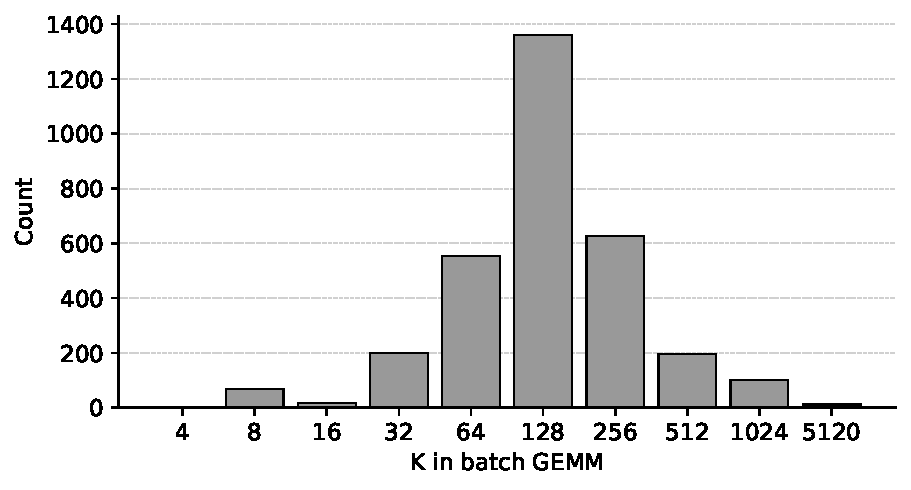
\includegraphics[width=\linewidth]{figures/shape_dist.pdf}
    \caption{Distribution of batched GEMM K dimensions over one Evoformer iteration of AlphaFold2 inference.}
    \label{fig:k_dist}
\end{figure}

Like other models based on transformers, the Evoformer is dominated by dense matrix multiplications: linear projections in attention, the Q/K/V/output GEMMs, the gated MLP that follows each attention block, and the bilinear updates inside the triangular multiplicative module. On an OPA architecture, the performance of these GEMMs is governed primarily by the reduction dimension $K$, for two reasons.

\textbf{Why $K$ matters on OPA.} Each MOPA instruction performs a rank-1 update directly into a ZA tile, so a complete GEMM tile is constructed by issuing $K$ MOPAs along the reduction axis and then \textit{draining} the tile back to memory. The drain step, which is absent from conventional FMA-based CPU GEMMs, is a fixed cost per output tile. As a result, the GEMM execution can be modelled as a four-stage pipeline: operand load, MOPA accumulation, tile drain, and writeback. The throughput is determined by how well MOPAs amortize the drain and writeback. When $K$ is large, the MOPA stage dominates and the kernel approaches peak compute throughput; when $K$ is small, drain and writeback occupy a comparable or larger fraction of the issue slots, and the kernel becomes memory- and instruction-bandwidth bound.

\textbf{The shape distribution in AlphaFold2.} Fig.~\ref{fig:k_dist} reports the distribution of $K$ across all batched GEMMs in a single Evoformer iteration. GEMMs with $K \le 256$ account for the dominant share of operator instances. This pattern is a direct consequence of AlphaFold2's small channel widths ($c_m, c_z \in \{128, 256\}$) and of attention being executed as batched per-head GEMMs with per-head dimension $c/N_{\text{heads}} = 32$ or $64$. The same hidden dimension that keeps the model parameter-efficient turns out to make every projection GEMM tall-and-skinny.

A small $K$ does not imply a small workload. These tall-and-skinny GEMMs typically come paired with large $M$, $N$, or batch dimensions. So their total FLOP count is comparable to, and often exceeds, that of the few large-$K$ GEMMs in the model. The optimization problem is how to make the OPA pipeline efficient at small $K$, which we address in Section~\ref{sec:optimizations}.

\subsubsection{Activation-Dominated Memory Pressure}
\label{sec:analysis:memory}

A second distinguishing property of AlphaFold2 is that its memory footprint is dominated by \textit{activations} rather than weights. With $c_m, c_z \le 256$, the parameter set is modest in size, but the intermediate tensors scale super-linearly in the input length:
\begin{itemize}
    \item the MSA representation grows as $O(N_s N_r c_m)$,
    \item the pairwise representation grows as $O(N_r^2 c_z)$,
    \item the attention logits ($Q K^\top$) grow as $O(N_s N_r^2)$ for MSA attention or $O(N_r^3)$ for triangular attention.
\end{itemize}

The cubic term is the binding constraint at long sequences. For example, when $N_r$ approaches a few thousand residues, a single triangular-attention logits tensor can consume tens of GiB, exceeding the on-package memory of many accelerators. The standard remedy is to chunk the attention computation along the batch or head dimension and stream tiles through fast memory.~\cite{zhao2024autochunk} Chunking trims peak memory linearly in the chunk size but it shrinks the per-tile workload exposed to parallel hardware.

% The implication for the 920F platform is two-sided. On one hand, the on-package memory is large enough that chunk sizes can remain comparatively generous, preserving more parallelism than a memory-constrained GPU could afford. On the other, once $N_r$ grows past the on-package capacity, the working set spills to off-chip memory and locality degrades---an effect that we observe directly in the long-sequence regime of our evaluation (Section~\ref{sec:end_to_end}).

\subsubsection{Frequent Tensor Layout Transformations}
\label{sec:analysis:comm}

The Evoformer is unusual among transformer architectures in that successive operators within the same block act along \textit{different} tensor axes. MSA row-wise attention contracts along the residue axis, MSA column-wise attention contracts along the sequence axis, and the triangular multiplicative module updates the pairwise tensor first along one residue axis and then along the other. To express each of these operators as a contiguous, vectorizable contraction, the implementation must transpose the underlying tensor between row-major and column-major layouts, which are marked $T$ and $T'$ in Fig.~\ref{fig:af2model}.

Each transposition has two costs on a many-core CPU. The first is data movement: transposing an MSA or pairwise activation touches every element of the tensor, and on a multi-NUMA node these elements are partitioned across local memories, so the transpose generates remote traffic that is bottlenecked by the inter-NUMA interconnect rather than by local DRAM bandwidth. The second is synchronization: when the workload is parallelized along the sequence or residue axis, every transpose acts as a barrier between the producers (which write along one axis) and the consumers (which read along the orthogonal axis). Both costs grow with activation size and therefore with sequence length.
Each block issues several layout transitions, and with 48 blocks per inference the cumulative cost becomes a non-trivial fraction of end-to-end runtime on long inputs. %The implication for our design is that minimizing the \textit{number} of transitions, and absorbing the residual ones into operator boundaries, is at least as important as accelerating the GEMMs themselves.

% \subsection{Summary}
% \label{sec:analysis:summary}

% The three bottlenecks above motivate a corresponding set of design decisions:
% \begin{enumerate}
%     \item Tall-and-skinny GEMMs require an OPA-aware kernel that aggressively amortizes the drain and writeback stages---addressed in Section~\ref{sec:optimizations} via a $K$-unblocked kernel and a tensor layout that matches the OPA operand format.
%     \item Activation-dominated memory pressure favours platforms with large on-package memory and rewards careful precision selection, which our FP16 mixed-precision strategy exploits.
%     \item Layout transpositions and NUMA traffic call for shared-memory communication primitives and a length-aware parallelism strategy that confines short sequences to a single NUMA node.
% \end{enumerate}

% The remainder of the paper develops these mechanisms in turn.
